\documentclass[11pt, oneside]{article}   	% use "amsart" instead of "article" for AMSLaTeX format
\usepackage{geometry}                		% See geometry.pdf to learn the layout options. There are lots.
\geometry{letterpaper}                   		% ... or a4paper or a5paper or ... 
%\geometry{landscape}                		% Activate for rotated page geometry
%\usepackage[parfill]{parskip}    		% Activate to begin paragraphs with an empty line rather than an indent
\usepackage{graphicx}				% Use pdf, png, jpg, or eps§ with pdflatex; use eps in DVI mode
								% TeX will automatically convert eps --> pdf in pdflatex		
\usepackage{amssymb}

\usepackage{fancyhdr}
\fancyhead[L]{DATE}
\fancyhead[C]{SE 3XA3 Test Plan}
\fancyhead[R]{Genzter}
\pagestyle{fancy}

\usepackage{float}

\usepackage{hyperref}

%SetFonts

%SetFonts


\title{Test Plan: Revision 0}
\author{Group 2 - Genzter \\
		\\ Binu, Amit - binua - 400023175
		\\ Bengezi, Mohamed - bengezim - 400021279
		\\ Samarasinghe, Sachin - samarya - 001430998
		\\Professor: Dr. Bokhari
		\\ Lab: L01}

\begin{document}
\maketitle

\newpage
\section{Revision History}

\begin{table}[h]
\begin{center}
\begin{tabular}{ | c | c | c | c | }
\hline
 Date & Version & Description & Author \\ 
\hline
 05/OCT/17 & 0.0 & Created Test Plan & Mohamed Bengezi, Amit Binu, Sachin Samarasinghe \\  
\hline
  & & & \\
\hline
 & & & \\
\hline 
 & & & \\ 
\hline 
\end{tabular}
\end{center}
\caption{Revision History}
\end{table}

\newpage
\tableofcontents
\listoffigures
\listoftables

\newpage
% INTRODUCTION
\section{Introduction}
\subsection{Purpose}
The goal of this project is to create a viable set of schedules for the user based on the inputted courses. All correcponding core's, labs, and tutorials must be included in each timetable. The automated testing shall include unit testing performed by the Mocha framework for javascript. Functional testing shall consist of input testing, along with conflict tests, and perfect input tests. Structural testing shall inlcude performance tests, such as a large number of courses as input, as well as dataset traversal tests. Fault and Mutation testing will occur throughout development. Manual testing, such as static testing, shall be done primarily by group code walkthrough's \& inspections, in order to check syntax and logic, and gain a better understanding of the program code as a whole. Dynamic testing shall include using a number of predetermined schedules from various programs, and using the courses on each schedule as input, and determining that each necessary core, lab, and tutorial are listed in the generated timetable. 

\subsection{Objectives}
This test plan will allow the team to head into the testing phase in an organized and informed manner, and with a clear goal in mind. These tests ensure that the product will be working as it should be when released for users. The plan will also ensure that testing is conducted properly, and any interested parties can learn about the testing of the product.\

\subsection{References}
Project inspiration: \url{http://timetablegenerator.io} \\
Open sourced similar project: \url{https://github.com/ash47/TimetableGenerator}

\newpage



% PLAN
\section{Plan}
\subsection{Software Description}
The program uses Node js for the backend, and HTML/CSS for the front end. The main modules in the program are the index.js module, which contains the code for the main page, the checkCourse.js module, which checks and  ensures all user inputs are valid and viable, the scheduler.js module, which is the main algorithm for creating the timetables, the Course.js module, which defines the course objects used throughout the program, and all the corresponding ejs files, which contain the HTML code for the front end of each page. 
%%%%%%%%%%%%%%%%%%%%%%%%%%%%%%

\begin{figure}[H] %  figure placement: here, top, bottom, or page
   \centering
   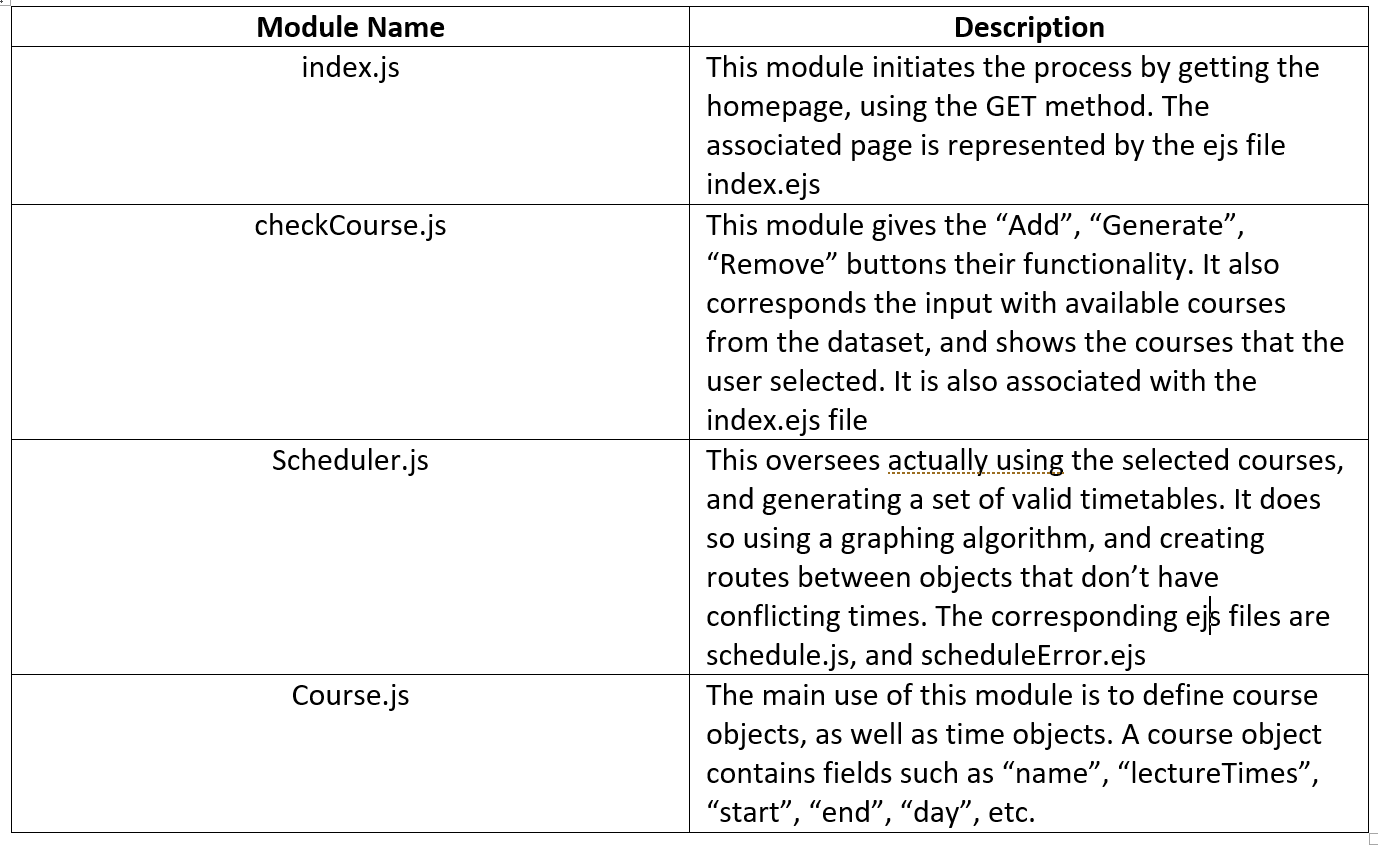
\includegraphics[width=5in]{Software_Description.png} 
   \caption{Software Description}
   \label{}
\end{figure}


\subsection{Test Team}
The entire Genzter team will be in tasked with testing. Testing shall be evenly divided between members.

\subsection{Automated Testing Approach}
As stated above, automated testing will be done using the javascript testing framework called \href{http://mochajs.org}{Mocha}. Accompanying Mocha will be an assertion library called \href{http://chaijs.com/}{Chai}. Unit tests will be set up, and the framework will be used to automatically run through all the unit tests, and reveal any faults that may reside in the program. The unit tests will include normal input, boundary cases, as well as extreme cases and conflicting cases. This will ensure that the program functions expectedly, and that no special cases were missed. In other words, this automated testing approach will make sure that in any case, the program will have a path to follow, and its behaviour can be predicted.

\subsection{Testing Tools}
For unit testing we will be using the testing framework \href{http://jasmine.github.io/}{Jasmine}. For system testing we will be running the game by executing it on a browser and observing the functionalities. For code analysis we will use humans with coding experience to analyze the code.

\subsection{Testing Schedule}
The testing schedule is included in the Gantt chart, located in the Project Schedule folder in the main directory.

\newpage

\section{System Test Description}
\subsection{Tests for Functional Requirements}
\subsubsection{Test Area 1 \\ Conflict Detection Test}
\begin{enumerate}
\item Type: Dynamic \\
Initial State: Homepage \\
Input: SFWRENG 3RA3, EARTHSC 2EI3 \\
Output: Conflict error page \\
The courses in the input field will be selected and added in the UI manually. The expected result, an error page, will be checked against the actual output. The courses selected must have conflicting time slots. \\

\item Type: Dynamic \\
Initial State: Homepage \\
Input: RELIGST-2TA3, SFWRENG 3BB4 \\
Output: Conflict error page \\
The courses in the input field will be selected and added in the UI manually. The expected result, an error page, will be checked against the actual output. The courses selected must have conflicting time slots. \\


\item Type: Dynamic \\
Initial State: Homepage \\
Input: BIOLOGY 2F03, SFWRENG 3MX3 \\
Output: Conflict error page \\
The courses in the input field will be selected and added in the UI manually. The expected result, an error page, will be checked against the actual output. The courses selected must have conflicting time slots. \\


\item Type: Dynamic \\
Initial State: Homepage \\
Input: MATLS 2B03, EARTHSC 2EI3 \\
Output: Conflict error page \\
The courses in the input field will be selected and added in the UI manually. The expected result, an error page, will be checked against the actual output. The courses selected must have conflicting time slots. \\
\end{enumerate}

\subsubsection{Test Area 2: Output Timetable}
\begin{enumerate}
\item Type: Manual \\
Initial State: Homepage \\
Input: SFWRENG 3XA3, SFWRENG 3BB4, SFWRENG 3DB3, SFWRENG 3MX3, COMMERCE 1AA3 \\
Output: Valid Schedule in a timetable format. \\
The courses in the input field will be selected and added in the UI manually. The expected result, a color coded schedule, will be checked against the actual output. Generated timetable must have every core, tutorial, lab etc. required for each course. It will be manually checked against the dataset and our own timetables \\

\item Type: Manual \\
Initial State: Homepage \\
Input:  ENGINEER-1C03, MATH-1ZC3, MATH-1ZB3,  ECON-1BB3, PHYSICS-1E03, MATLS-1M03 \\
Output: Valid Schedule in a timetable format. \\
The courses in the input field will be selected and added in the UI manually. The expected result, a color coded schedule, will be checked against the actual output. Generated timetable must have every core, tutorial, lab etc. required for each course. It will be manually checked against the dataset and our own timetables \\

\item Type: Manual \\
Initial State: Homepage \\
Input: RELIGST-2TA3, RELIGST-2QQ3, POLSCI-2I03, POLSCI-4CA3\\
Output: Valid Schedule in a timetable format. \\
The courses in the input field will be selected and added in the UI manually. The expected result, a color coded schedule, will be checked against the actual output. Generated timetable must have every core, tutorial, lab etc. required for each course. It will be manually checked against the dataset and our own timetables \\

\item Type: Manual \\
Initial State: Homepage \\
Input:EARTHSC-2EI3, EARTHSC-2C03, GEOG-2UI3, GEOG-2GI3, BIOLOGY-2F03\\
Output: Valid Schedule in a timetable format. \\
The courses in the input field will be selected and added in the UI manually. The expected result, a color coded schedule, will be checked against the actual output. Generated timetable must have every core, tutorial, lab etc. required for each course. It will be manually checked against the dataset and our own timetables \\
\end{enumerate}

\subsubsection{Regression Testing}
Regression testing will continually happen to ensure all features continue to function ideally, no matter the changes occuring to the program.

\subsubsection{Parallel Testing}
Please refer to \hyperref[sec:compare]{this section}

\subsection{Tests for Non-functional Requirements}
\subsubsection{Test Area 1: Speed Performance}
\begin{enumerate}

\item Type: Manual \\
Initial State: Homepage \\
Input: SFWRENG 3XA3, SFWRENG 3BB4, SFWRENG 3DB3, SFWRENG 3MX3, COMMERCE 1AA3 \\
Output: Schedule in a timetable format. \\
The input courses shall be selected, and the the generator is timed from when the "Generate" button is pressed. \\

\item Type: Manual \\
Initial State: Homepage \\
Input:  ENGINEER-1C03, MATH-1ZC3, MATH-1ZB3,  ECON-1BB3, PHYSICS-1E03, MATLS-1M03 \\
Output: Schedule in a timetable format. \\
The input courses shall be selected, and the the generator is timed from when the "Generate" button is pressed.  \\
\end{enumerate}

\subsubsection{Test Area 2: UI}
\begin{enumerate}

\item Type: Manual \\
Initial State: Homepage \\
Input: Any McMaster Course \\
Output: Add course to list of courses \\
Any McMaster course is selected, and the "Add" button is pressed. This is to test the ability of the UI to retrieve input from the user. \\

\item Type: Manual \\
Initial State: Homepage with list of courses chosen\\
Input:  Pressing the "Remove" button \\
Output: Removal of the selected course \\
Starting off with a list of courses, the "Remove" button will be pressed to test the ability of the UI to modify the course list at the request of the user.  \\


\item Type: Manual \\
Initial State: Homepage with list of courses chosen\\
Input:  Pressing the "Generate" button \\
Output: Timetable \\
Starting off with a list of courses, the "Generate" button will be pressed to test the ability of the UI to display output at the request of the user.  \\
\end{enumerate}

\subsubsection{Test Area 3: Maintainability}
\begin{enumerate}
\item Type: Static \\
Initial State: Not running \\
Input: Code walkthrough and inspection\\
Output: N/A  \\
This test is a static test for confirming the syntax and structural integrity of the backend of the program.\\
\end{enumerate}


\subsubsection{Traceability}
CHECK WITH T/A UVCFDTXCFVGUBINOUBVYCFTDXRTCFYGVUBHINJKML;PNOBIUVTYCRX
\newpage

\section{PoC Test}

\subsection{Test Area 2: Conflict Detection}
\begin{enumerate}
\item Type: Dynamic \\
Initial State: Homepage \\
Input: BIOLOGY 2F03, SFWRENG 3MX3 \\
Output: Conflict error page \\
The courses in the input field will be selected and added in the UI manually. The expected result, an error page, will be checked against the actual output. The courses selected must have conflicting time slots. \\
\end{enumerate}

\subsection{Test Area 1: Schedule Output}
\begin{enumerate}
\item Type: Manual \\
Initial State: Homepage \\
Input: SFWRENG 3XA3, SFWRENG 3BB4 \\
Output: Valid Schedule in a timetable format. \\
The courses in the input field will be selected and added in the UI manually. The expected result, a color coded schedule, will be checked against the actual output. Generated timetable must have every core, tutorial, lab etc. required for each course. It will be manually checked against the dataset and our own timetables \\
\end{enumerate}

\section{Comparison to Existing Implementation}\label{sec:compare}
The project will be benchmarked against two existing implementations, \url{http://timetablegenerator.io} and \url{https://github.com/ash47/TimetableGenerator}. Mainly, we will be comparing our project with \url{http://timetablegenerator.io} because it uses the McMaster database as well, so we can fully compare the generated timetables. The outputs are fairly similar, so comparison should not be very difficult. The comparison will be done manually by the testing team.
\section{Unit Testing Plan}
ASK TA ABOUT THUS DBUIEWBVHBEODIWEEOP
\end{document}
